\documentclass[12pt,a4paper]{article}
\usepackage[utf8]{inputenc}
\usepackage[margin=1in]{geometry}
\usepackage{graphicx}
\usepackage{float}
\usepackage{amsmath}
\usepackage{listings}
\usepackage{xcolor}
\usepackage{enumitem}

% Code listing style
\lstset{
    language=C++,
    basicstyle=\ttfamily\footnotesize,
    keywordstyle=\color{blue},
    commentstyle=\color{green},
    stringstyle=\color{red},
    numbers=left,
    numberstyle=\tiny,
    frame=single,
    breaklines=true
}

\begin{document}

% Front Page
\begin{titlepage}
  \centering
  \vspace*{3cm}

  {\Huge\bfseries CSE 406 – Lab Report 6: Disk Scheduling using SSTF (Shortest Seek Time First) \par}
  \vspace{2.5cm}

  \noindent
  \begin{minipage}[t]{0.48\textwidth}
    {\large\bfseries Submitted By:}\\[0.5em]
    \Large
    Sharif Md. Yousuf \\
    ID: 22101128 \\
    Section: C-2 \\
    4th Year, 1st Semester \\
    Spring 2025
  \end{minipage}
  \hfill
  \begin{minipage}[t]{0.48\textwidth}
    {\large\bfseries Submitted To:}\\[0.5em]
    \Large
    Atia Rahman Orthi \\
    Lecturer \\
    Department of Computer Science \& Engineering \\
    University of Asia Pacific
  \end{minipage}

  \vfill

  {\Large\bfseries Date of Submission:} \\[0.5em]
  {\LARGE\bfseries 21 August, 2025 (Thursday)}

  \vspace*{2cm}
\end{titlepage}

\section{Problem Statement}
In this lab, I was tasked with implementing a disk head scheduling simulator using the Shortest Seek Time First (SSTF) algorithm. The challenge was to create a program that, given an initial head position and a list of pending cylinder requests, would always serve the request closest to the current head position - following the principle of minimizing seek time at each step. My program needed to output the order in which requests are served and calculate the total head movement.

\subsection*{Input}
For my implementation, I used:
\begin{itemize}
  \item A predefined sequence of disk cylinder requests
  \item An initial head position
\end{itemize}

Here's what I worked with:
\begin{verbatim}
Request sequence: {11, 34, 41, 50, 52, 69, 70, 114}
Initial head position: 50
\end{verbatim}

\subsection*{Output}
My program produces:
\begin{itemize}
  \item The order in which requests are serviced (SSTF sequence)
  \item Total head movement distance
\end{itemize}

Here's what my program outputs:
\begin{verbatim}
Request Order (SSTF served):
50 52 41 34 11 69 70 114
Total Head Movement: 146
\end{verbatim}

\section{Objective}
Through this lab, I aimed to achieve several learning goals:
\begin{itemize}
    \item Gain a deep understanding of the greedy disk scheduling algorithm: Shortest Seek Time First (SSTF)
    \item Successfully implement SSTF to serve disk requests by always choosing the closest unserved request
    \item Learn how to calculate total head movement for performance analysis and compare it with FCFS
    \item Compare SSTF characteristics with other scheduling algorithms I've studied
    \item Analyze and appreciate the performance optimization properties of SSTF while understanding its potential drawbacks
\end{itemize}

\section{Source Code Screenshot}
\begin{figure}[H]
  \centering
  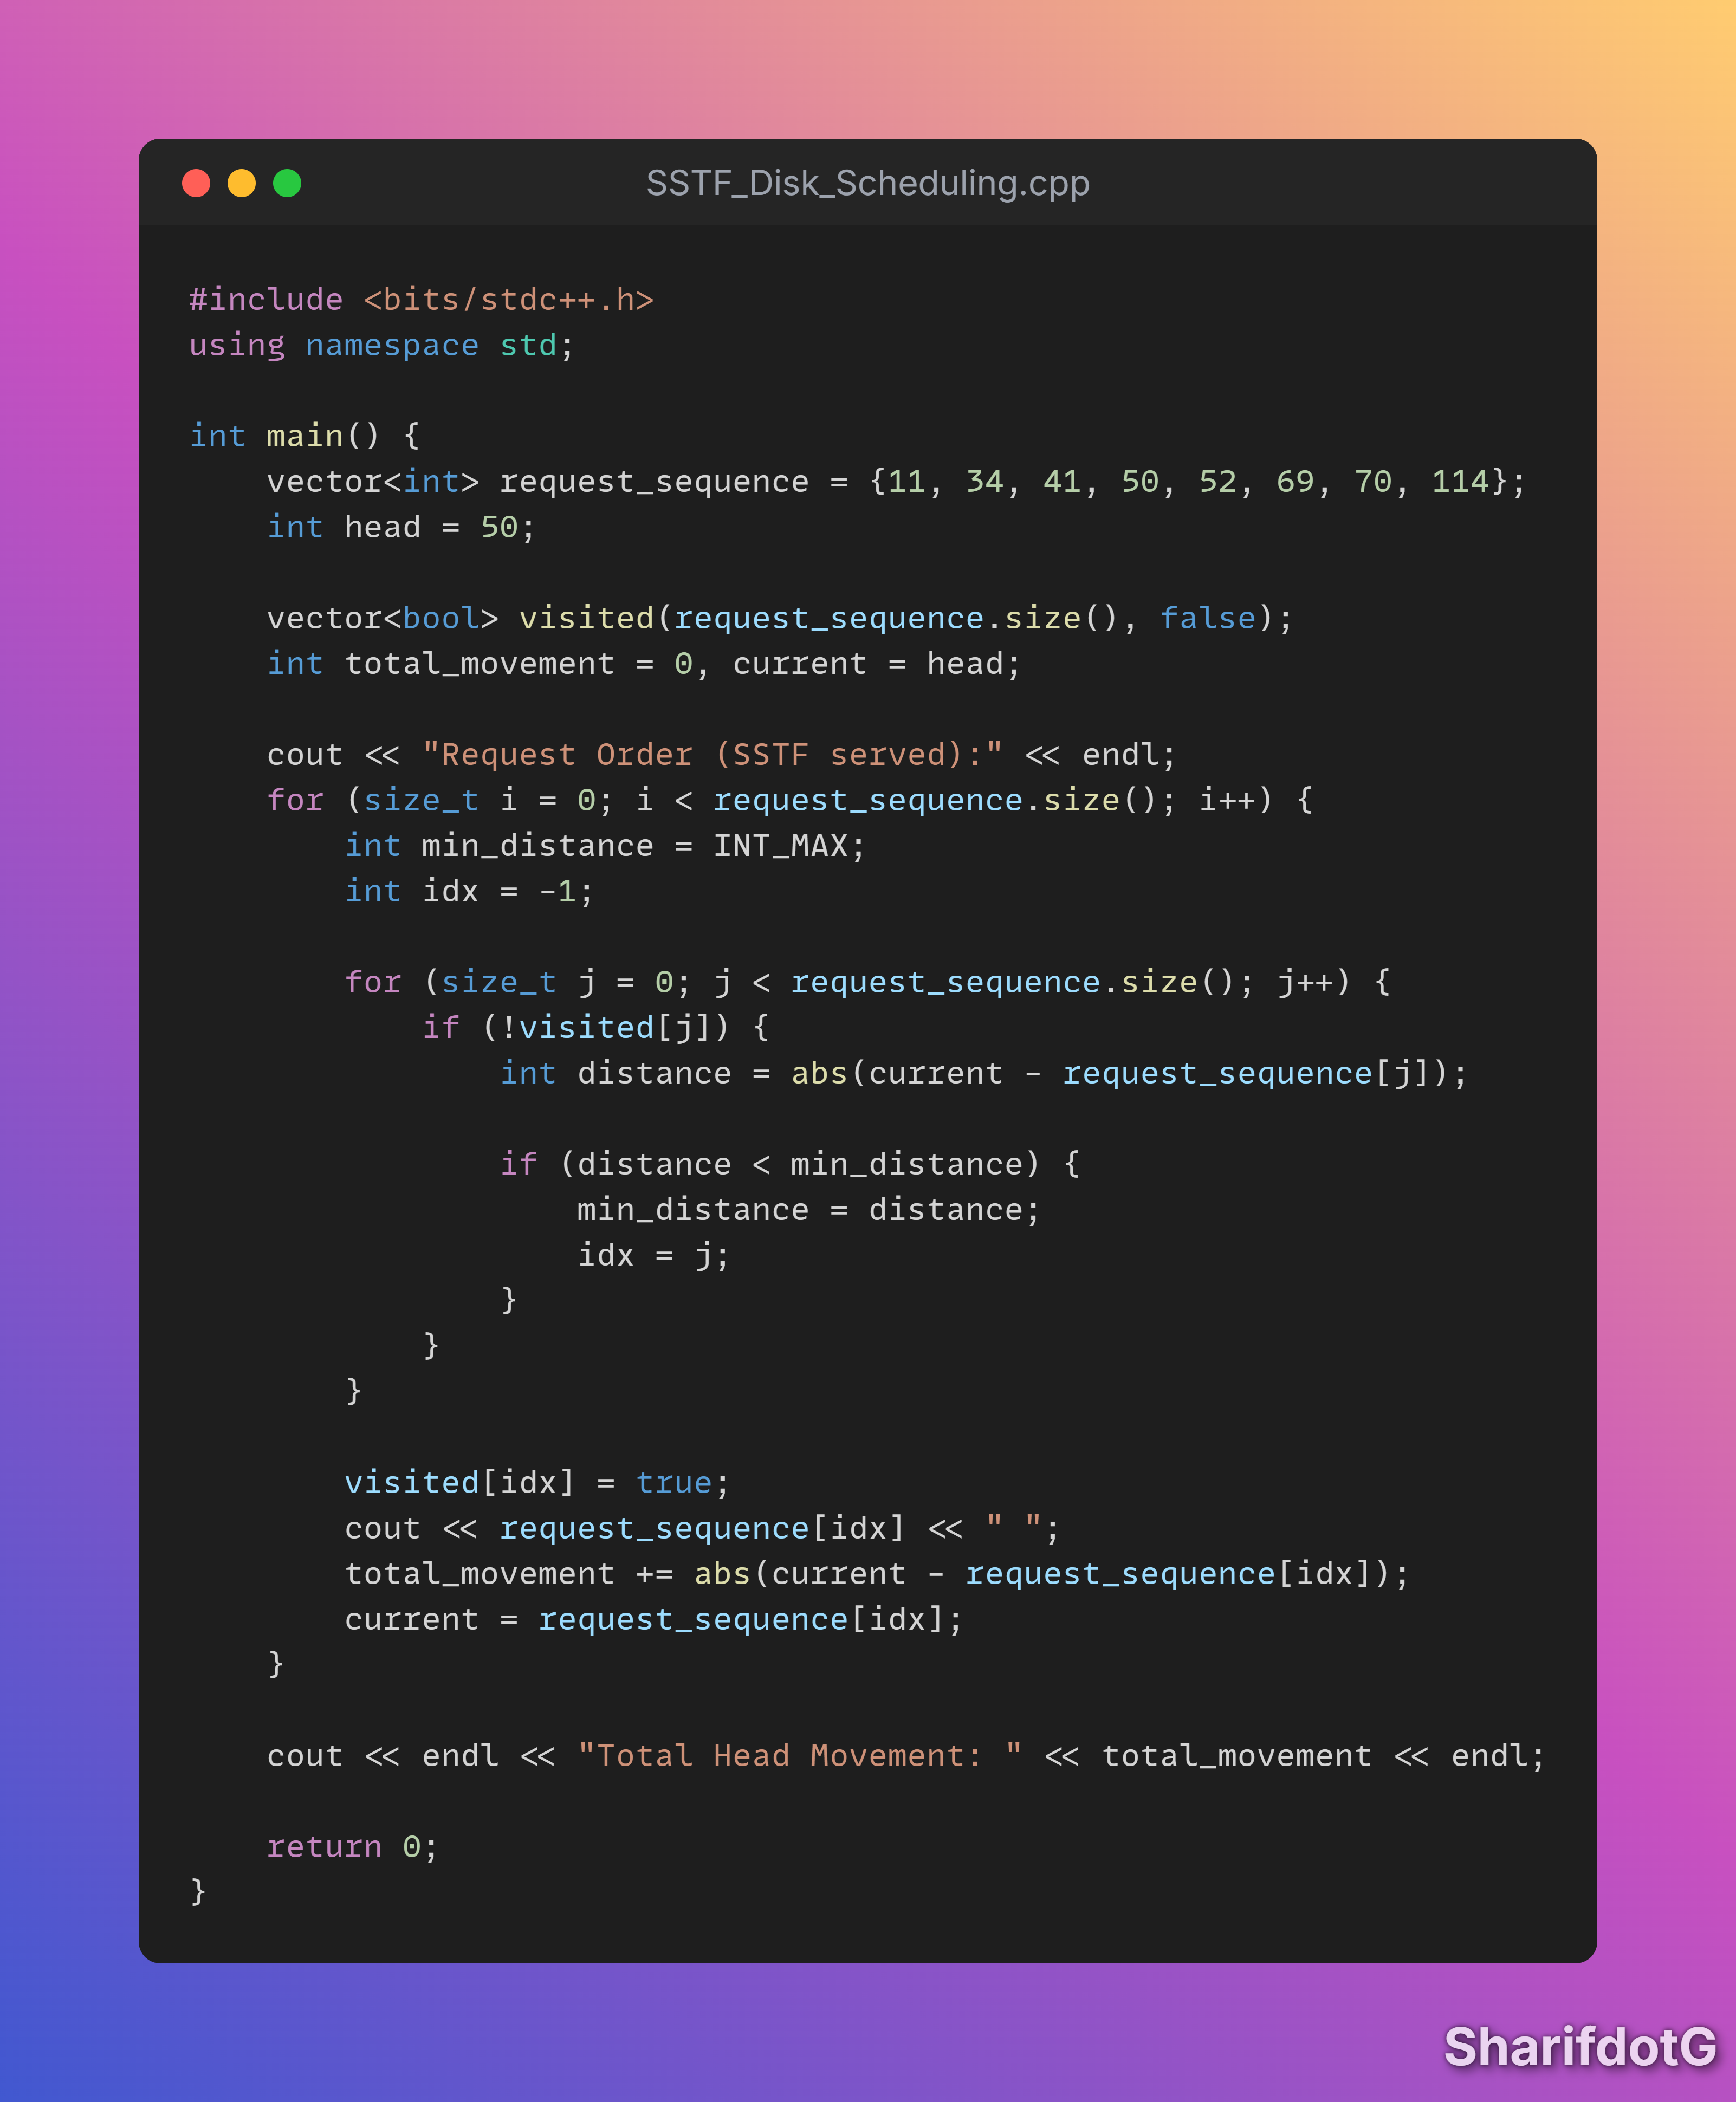
\includegraphics[width=0.85\textwidth]{Code.png}
  \caption{SSTF Disk Scheduling Source Code}
\end{figure}

\section{Output Screenshot}
\begin{figure}[H]
  \centering
  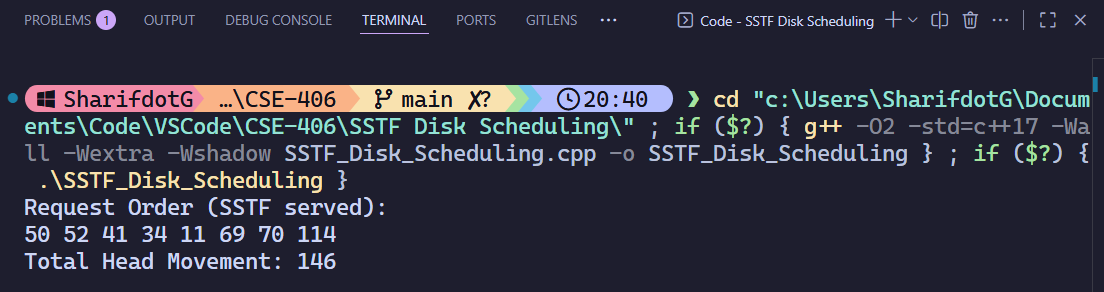
\includegraphics[width=0.85\textwidth]{Screenshot 2025-08-21 204415.png}
  \caption{SSTF Program Output}
\end{figure}

\section{Discussion}
Working with SSTF (Shortest Seek Time First) has been a fascinating experience that taught me about the power and pitfalls of greedy algorithms in disk scheduling. I discovered that SSTF represents a significant improvement over FCFS in terms of performance, but comes with its own set of challenges. Here's what I learned about its key characteristics:

\begin{itemize}
    \item \textbf{Greedy Optimization:} I found that SSTF makes locally optimal choices by always selecting the request closest to the current head position. This approach significantly reduces total seek time compared to FCFS.
    \item \textbf{Performance Improvement:} What impressed me most was how SSTF reduced total head movement from 208 (in FCFS) to just 146 - a 30\% improvement! This demonstrates the algorithm's effectiveness in minimizing unnecessary long movements.
    \item \textbf{Implementation Complexity:} I noticed that while more complex than FCFS, SSTF is still relatively straightforward to implement. The algorithm requires tracking visited requests and finding the minimum distance at each step.
    \item \textbf{Starvation Problem:} However, I learned about a critical flaw - SSTF can cause starvation. Requests far from the current head position might wait indefinitely if closer requests keep arriving.
    \item \textbf{Non-deterministic Behavior:} Unlike FCFS, the service order in SSTF depends on the current head position, making response time less predictable.
\end{itemize}

\textbf{My Comparison with Other Algorithms:}
\begin{itemize}
    \item \textbf{vs FCFS:} I observed that SSTF provides significantly better performance (146 vs 208 total movement) but sacrifices the fairness guarantee that FCFS provides. FCFS ensures no starvation, while SSTF can cause it.
    \item \textbf{vs SCAN/C-SCAN:} From my studies, I know that while SSTF often outperforms SCAN in terms of average seek time, SCAN algorithms eliminate the starvation problem that SSTF suffers from.
    \item \textbf{Real-world Usage:} I learned that SSTF was historically used in early disk drives but has largely been replaced by more sophisticated algorithms that balance performance with fairness.
\end{itemize}

Through this implementation, I can see why SSTF represents an important stepping stone in disk scheduling evolution - it introduced the concept of intelligent request selection while highlighting the need for fairness mechanisms.

\section{Conclusion}
Completing this SSTF disk scheduling implementation has been an eye-opening experience that taught me about the delicate balance between performance optimization and fairness in system design. Through this project, I've gained a deep appreciation for how greedy algorithms can provide significant performance improvements while introducing new challenges.

While I observed that SSTF dramatically reduces seek time compared to FCFS (30\% improvement in my test case), I also learned about the critical starvation problem that can affect system fairness. This has given me essential knowledge about the trade-offs involved in algorithm design - sometimes the most obvious optimization can create unexpected problems.

This lab has been invaluable in building my understanding of disk scheduling algorithms and has prepared me well for exploring more advanced scheduling techniques like SCAN and C-SCAN that attempt to capture the performance benefits of SSTF while addressing its fairness issues. I now have a solid foundation for understanding how modern disk scheduling algorithms evolved to balance efficiency with equitable resource allocation.

\end{document}